\documentclass[a4paper, 11pt]{article}
\usepackage{amsmath}
\usepackage{graphicx}
\usepackage{geometry}
\usepackage{listings}
\usepackage[colorlinks,linkcolor=red]{hyperref}
\geometry{scale=0.8}

\title{	
\normalfont \normalsize
\textsc{School of Data and Computer Science, Sun Yat-sen University} \\ [25pt] %textsc small capital letters
\rule{\textwidth}{0.5pt} \\[0.4cm] % Thin top horizontal rule
\huge  E01 Maze Problem\\ % The assignment title
\rule{\textwidth}{2pt} \\[0.5cm] % Thick bottom horizontal rule
\author{19214808 Yikun Liang}
\date{\normalsize\today}
}

\begin{document}
\maketitle
\tableofcontents
\newpage
\section{Task}



\begin{itemize}
	\item Please solve the maze problem (i.e., find the shortest path from the start point to the finish point) by using BFS or DFS (Python or C++)
	\item The maze layout can be modeled as an array, and you can use the data file \texttt{MazeData.txt} if necessary.
	\item Please send \texttt{E01\_YourNumber.pdf} to \texttt{ai\_2020@foxmail.com}, you can certainly use \texttt{E01\_Maze.tex} as the \LaTeX template.
\end{itemize}

\begin{figure}[ht]
\centering
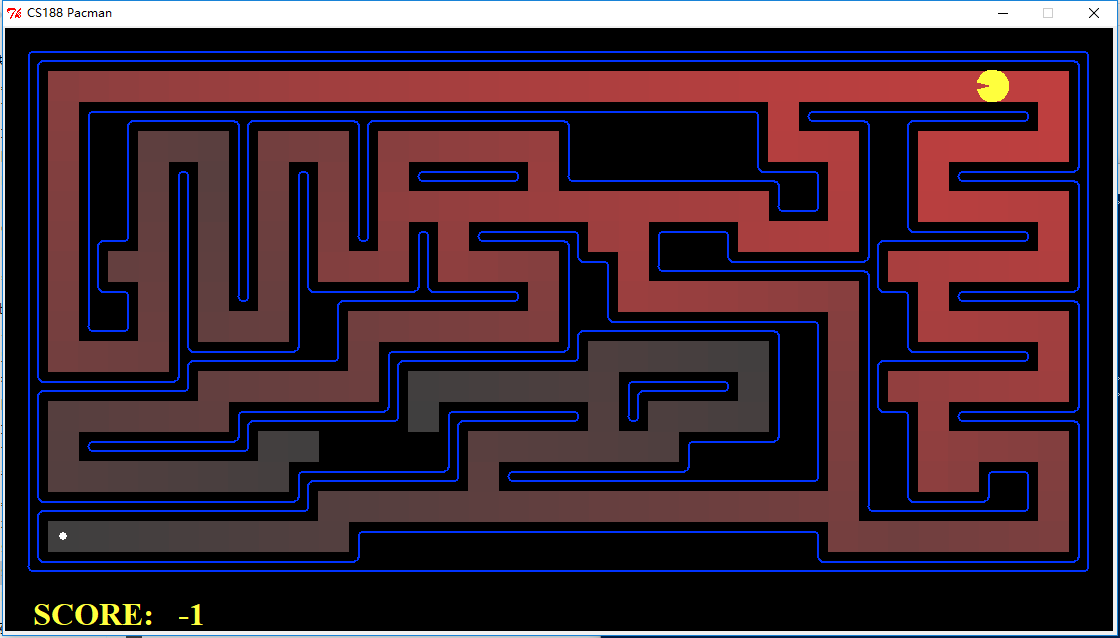
\includegraphics[width=15cm]{Pic/Pacman}

\caption{Searching by BFS or DFS}
\end{figure}
\section{Codes}
%%\lstset{language=C++}
\lstset{language=Python, frame=single}
\begin{lstlisting}
import queue
directions = ((-1, 0), (1, 0), (0, -1), (0, 1))
def bfs(q, maze):
    while True:
        cur = q.get()
        for direction in directions:
            next = (cur[0] + direction[0], cur[1] + direction[1])
            # This is used to avoid crossing the boundary.
            try:
                next_val = maze[next[0]][next[1]]
            except:
                continue
            ''' This is used to log last point's position,
            in order to prevent the process from visiting a point twice,
            and to jot down paths.'''
            if next_val == '0':
                maze[next[0]][next[1]] = cur
                q.put(next)
            elif next_val == 'E':
                maze[next[0]][next[1]] = cur
                return next
def read_maze(maze):
    with open("MazeData.txt") as f:
        while True:
            line = f.readline()
            if not line:
                break
            maze.append(list(line))
def init_queue(q):
    for i in range(len(maze)):
        for j in range(len(maze[i])):
            if maze[i][j] == 'S':
                q.put((i, j))
def print_path(maze):
    path = list()
    path.append(end)
    while True:
        cur = maze[path[-1][0]][path[-1][1]]
        if cur == 'S':
            break
        path.append(cur)
    while path:
        cur = path.pop()
        print(cur, end = '')
maze = list()
read_maze(maze)
q = queue.Queue()
init_queue(q)
end = bfs(q, maze)
print_path(maze)
\end{lstlisting}

\section{Results}
\begin{figure}[ht]
\centering
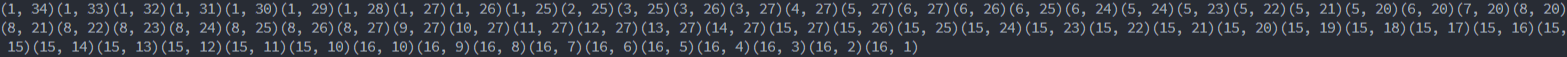
\includegraphics[width=15cm]{result.png}
\caption{Results}
\end{figure}


%\clearpage
%\bibliography{E:/Papers/LiuLab}
%\bibliographystyle{apalike}
\end{document} 